%Typische Problem  Dreiecksmassig

%In der GPU-Programmierung kann mann auch viele Probleme treffen.

%\subsection{Dreieckförmige Summation}
%Ein typisches Problem ist Bloksummation. Aus der Beschreibungen der Operationen Multiplikationen der Matrix mal Vektor und Sparsematrize  mal Vektor beruhen obige Operationen auf Vektormultiplikationen, die schließlich ein Summierungsverfahren in jedem Block enthalten. Blocksummation in einzigen Thread ist nicht effizient. Die einführende Algorithmus: Dreieckförmige Summation lautet wie Fig.\ref{Dreieck} . In erst Schritte werden 2n und 2n+1 Elements des Produktvektors $cs$ in jeweilig Threads summiert. In zweiter Schritte werden 4n und 4n+2 Elements summiert. Bis BlockSize/2 Schritte erhalt man endlich Ergebnisse.

\subsection{Summation längs eines Vektors}

Als typisches Teilproblem tritt die Summation der Vektorelemente zu
einem Skalar auf, bspw. beim Skalarprodukt und bei der Matrizenmultiplikation.
Der klassische Ansatz, die Addition als Schleife mit einem Akkumulator
auszuführen, wäre ineffizient weil nur ein einziger Thread für die
Arbeit benutzt werden könnte.
Abb. \ref{Dreieck} zeigt schematisch ein Verfahren mit mehreren Threads
die Teilergebnisse aufsummieren.
Die Grundidee: im ersten Schritt die Elemente
$cs_{2n}$ und $cs_{2n+1}$ summiert.
Im zweiten Schritt $cs_{4n}$ und $cs_{4n+1}$. Für die Errechnug
des Ergebnisses benötigt man $ \log_2(blocksize)$ Iterationsschritte.

\begin{figure}[htbp]
%\centering
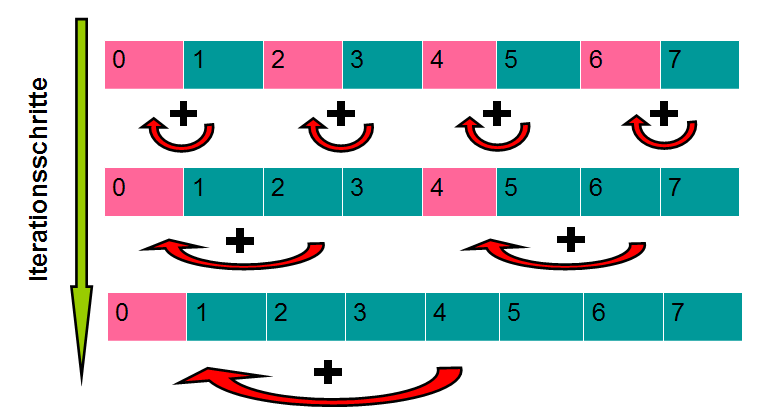
\includegraphics[width=3.5in]{../xby/pic//dreieck}
\caption{\label{Dreieck}Dreieckförmige Summation, Iterationsschritte von oben nach unten.}
\end{figure}

Beispielcode und eine detaillierte Beschreibung findet man in \cite{reduction}.

%%Dreieckmassig code zeigen
\begin{verbatim}
#define BLOCK_EXP 9
#define DEF_BLOCKSIZE 1 << BLOCK_EXP
short offset = 1;
for (short i = 1;i < BLOCK_EXP; i++) {
    short old = offset;
    offset <<= 1;
    if (threadIdx.x % offset == 0) {
        Vs[threadIdx.x] += Vs[threadIdx.x
        										+ old];
    }
    __syncthreads();
}
if (threadIdx.x == 0) {
    out[0] = Vs[0] + Vs[offset];
}
\end{verbatim}
